\chapter{Implementacja}

\section{Zastosowane technologie}

Wybór technologii użytych w implementacji został podyktowany jej architekturą --- interfejs użytkownika dostępny jest tylko i wyłącznie w przeglądarce internetowej, z tego powodu wybrane przez autora i opisane poniżej narzędzia są kojarzone jedynie w obszarze technologii internetowych. Interfejs graficzny wywarł niemały wpływ na wybór narzędzi, z uwagi na fakt, że osoba korzystająca z aplikacji powinna w łatwy i intuicyjny sposób:

\begin{itemize}[noitemsep]
  \item poruszać się po katalogach, plikach oraz wątkach,
  \item wyszukiwać wątki, komentarze lub pojedyncze słowa wewnątrz nich,
  \item wydzielić te wątki, które najbardziej interesują użytkownika,
  \item przeglądać statystyki dotyczące wpisywanych komentarzy.
\end{itemize}

Narzędzie, które zostało wybrane do realizacji tych zadań to AngularJS \cite{angular} --- technologia ułatwiająca kontrolę nad elementami interfejsu, stworzona w języku JavaScript. Jednakże, aby cały system prawidłowo i sprawnie działał, potrzebna była również technologia, która umożliwia przekazanie do interfejsu danych w odpowiedniej formie, pobranie z niego zadań wyznaczonych przez użytkownika i odpowiednie ich zrealizowanie. Do tych celów użyto języka Python \cite{python} wraz z narzędziem o nazwie Django \cite{django} do implementacji aplikacji internetowych. Połączenie Python/Django oraz AngularJS okazało się wystarczające do stworzenia aplikacji --- poza nimi użyte zostały wyłącznie skrypty odpowiadające za wygląd interfejsu.

\subsection*{AngularJS}

AngularJS jest otwartą biblioteką języka JavaScript, która została stworzona w 2009 roku i obecnie jest wspierana przez firmę Google. Najważniejszą funkcją narzędzia jest dwukierunkowe wiązanie danych (tzw. ,,emph{two-way data binding}''), które wyjątkowo łatwo obsługuje się wewnątrz szablonów HTML --- za ich pomocą zmiany wewnątrz modelu są natychmiast odzwierciedlone w interfejsie i na odwrót: elementy wprowadzone bądź zmienione przez użytkownika natychmiastowo znajdują odzwierciedlenie w modelu.

Biblioteka korzysta z wzorca MVC (Model-View Controller), aby ułatwić nie tylko implementację, ale również testowanie tworzonego systemu. AngularJS umożliwia bardzo łatwe zarządzanie dynamiczną treścią poprzez wspomniane wcześniej szablony i dodatkowe komendy wewnątrz szablonów. Dynamika aplikacji zaimplementowanej w niniejszej pracy była głównym wyzwaniem podczas jej tworzenia, a biblioteka AngularJS znacząco wpłynęła zarówno na poprawność, jak i objętość kodu.

\subsection*{Django}

O ile AngularJS został wykorzystany w znacznej mierze, o tyle stopień wykorzystania funkcjonalności Django został zredukowany do minimum. Biblioteka Django jest biblioteką do kompleksowego budowania stron internetowych w dowolnych architekturach (np. REST \cite{rest}), stworzoną, by jak najbardziej automatyzować kod i jak najszybciej --- a zarazem jak najprościej --- tworzyć skomplikowane serwisy. Narzędzie użyte zostało do implementacji z uwagi na prostotę i możliwości testowania, debugowania oraz możliwości rozbudowania zaimplementowanej aplikacji o dodatkowe rozwiązania.

Biblioteka Django powstała w 2003 roku, stworzona została przez programistów związanych ze środowiskiem dziennikarskim, dzięki czemu przystosowana jest do szybkiej i nieskomplikowanej pracy. Podobnie jak AngularJS pozwala (poprzez mechanizm szablonów) na łatwe i intuicyjne umieszczanie dynamicznych elementów na stronie. Wybrana została głównie ze względu na swoją prostotę oraz dodatkowe funkcjonalności ułatwiające pracę nad aplikacją np. możliwość automatycznego ponownego uruchamiania serwera podczas wprowadzania w nim zmian (co jest robione automatycznie).

\section{Komunikacja z serwerem}

Komunikacja między klientem a serwerem odbywa się poprzez zapytania \texttt{HTTP}, wewnątrz których przesyłane są dane potrzebne zarówno stronie klienta do ich wyświetlenia, jak i stronie serwera do wprowadzenia ich do systemu. Poniżej dokładnie opisane zostaną operacje wykonywane przez serwer, podzielone na grupy ze zbliżonym obszarem funkcjonalności.

\subsection{Foldery}

Operacje dostępne dla folderów w aplikacji TeamSync zostały ograniczone do dodawania ich oraz usuwania. Dodatkowe okna z ustawieniami, edycja folderów zostały przewidziane jako ewentualną dalszą rozbudowę systemu. W pracy skupiono się na pełnowartościowym korzystaniu z podstawowej funkcjonalności (synchronizacja danych oraz wprowadzanie komentarzy), co zostało spełnione bez konieczności implementacji edycji folderów.

\subsubsection*{Pobieranie listy folderów}

\begin{figure}[h!]
  \vspace{5pt}
  \begin{center}
    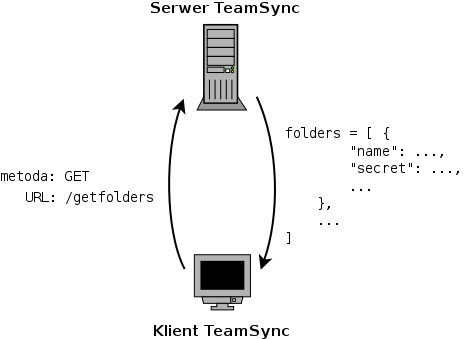
\includegraphics[width=250pt]{figures/metgetfolders.png}
  \end{center}
  \caption{Komunikacja w systemie \emph{TeamSync} podczas wywoływania metody \texttt{getfolders} --- pobieranie listy folderów.}
  \label{picmetgetfolders}
\end{figure}

Aby umożliwić użytkownikowi wybór folderu z listy synchronizowanych katalogów, aplikacja przeglądarkowa wysyła do serwera zapytanie \texttt{HTTP} za pomocą metody \texttt{GET} na adres \texttt{http://<adres oraz port serwera TeamSync>\-/getfolders}. Odpowiedź z serwera umieszczana jest wewnątrz listy \texttt{folders}, która przechowuje informacje dotyczące katalogów zapisane w formacie \texttt{JSON}.

\begin{figure}[htb!]
\label{newcommentrequest}
  \begin{verbatim}
          [
              {
                  "name": "testowy katalog", 
                  "dir": "/home/user/testowy katalog", 
              
                /* wartości mniej istotne, pobrane podczas
                   wykonywania metody get_folders takie jak: size,
                   down_speed, up_speed, error, indexing, id, type */
         
                  "secret": "A3LL43HJ257YCKMOLAD7QSEAS7U373BVO", 
                  "identity": "Filip Rachwalak", 
                  "uid": "FWZPQQKUE3JPQKWY557FERJ4SD3BSFMM", 
                  "users": [
                      {
                          "uid": "PWGGJTDPC35O43SLEKFPBPIG3NYV7PH7", 
                          "identity": "Jan Iksiński"
                      }, 
                      {
                          "uid": "FWZPQQKUE3JPQKWY557FERJ4SD3BSFMM", 
                          "identity": "Filip Rachwalak (Ty)"
                      }
                  ]
              }
          ]
  \end{verbatim}
  \caption{Przykładowa odpowiedź serwera na żądanie pobrania listy synchronizowanych folderów.}
\end{figure}

W odpowiedzi serwera znajdują się wszystkie informacje dotyczące folderów otrzymane z BitTorrent Sync API (w sekcji \ref{btsyncapiproto} znajduje się dokładne wyjaśnienie zwracanych danych przez metodę \texttt{get\_folders}) z dodatkowymi danymi:

\begin{itemize}[noitemsep]
  \item \emph{name} --- ułatwia interfejsowi wyświetlanie nazwy katalogu w liście,
  
  \item \emph{identity} oraz \emph{uid} --- tożsamość i identyfikator użytkownika,
  
  \item \emph{users} --- lista użytkowników zawierająca ich identyfikatory oraz tożsamości, potrzebna do wyświetlania wszystkich użytkowników w folderze oraz autorów komentarzy. Wartości wewnątrz tej listy są pobrany z katalogu \texttt{.Users} wewnątrz folderu współdzielonego.
\end{itemize}

W powyższym przykładzie użytkownik o identyfikatorze \texttt{FWZPQQKU\-E3JPQKWY\-557FERJ4\-SD3BSFMM} i tożsamości \texttt{Filip Rachwalak} posiada tylko jeden współdzielony folder, który dzieli z użytkownikiem \texttt{Jan Iksiński} o identyfikatorze \texttt{PWGGJTDP\-C35O43SL\-EKFPBPIG3\-NYV7PH7}. Bezpośrednia ścieżka katalogu to \texttt{/home/user/\-testowy katalog}, natomiast nazwa, jaka będzie wyświetlana na liście w przeglądarce to \texttt{testowy katalog}. \emph{Secret} folderu to \texttt{A3LL43HJ2\-57YCKMOL\-AD7QSEAS7\-U373BVO}.

\subsubsection*{Tworzenie folderu}

\begin{figure}[h!]
  \vspace{5pt}
  \begin{center}
    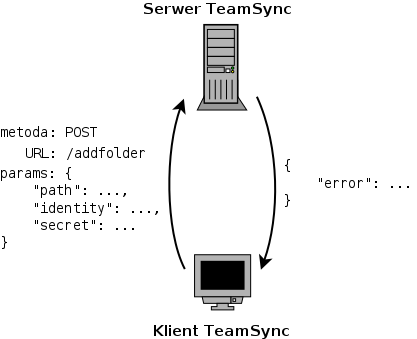
\includegraphics[width=230pt]{figures/metaddfolder.png}
  \end{center}
  \caption{Komunikacja w systemie \emph{TeamSync} podczas wywoływania metody \texttt{addfolder} --- tworzenie folderu.}
  \label{picmetgetfolders}
\end{figure}

Użytkownik ma możliwość wyboru pomiędzy rodzajem dodawanego katalogu --- inicjacja własnego lub dołączenie do już istniejącego, stworzonego przez innego użytkownika folderu. Podczas obydwóch tych operacji przeglądarkowy interfejs graficzny wysyła do serwera zapytanie metodą \texttt{POST} na adres \texttt{http://<adres oraz port serwera TeamSync>\-/addfolder}. W parametrach żądania znajdują się:

\begin{itemize}[noitemsep]
  \item \emph{path} --- bezwzględna ścieżka do folderu, którego zawartość od tej pory będzie synchronizowana z pozostałymi użytkownikami,
  
  \item \emph{identity} --- zadeklarowana przez użytkownika tożsamość, czyli nazwa użytkownika, jaka będzie wyświetlana innym węzłom,
  
  \item \emph{secret} --- za jego pomocą BitTorrent Sync odnajdzie w sieci pozostałych użytkowników; jeśli ten parametr pozostanie pusty, serwer stworzy nowy folder (nie w fizycznym sensie, lecz w logicznym --- doda podany w parametrze \emph{path} folder do folderów współdzielonych).
\end{itemize}

Serwer otrzymując żądanie z powyższymi parametrami, przekazuje je poprzez zapytanie \texttt{HTTP} do BitTorrent Sync API, za pomocą funkcji \texttt{add\_folder} (dokładny opis metody znajduje się w sekcji \ref{btsyncapiproto}). Jeśli podstawowa walidacja wprowadzanych danych się nie powiedzie, lub jeśli BitTorrent Sync API zwróci błąd, serwer oprócz zwrócenia odpowiedzi z treścią błędu nie wykona żadnych dodatkowych instrukcji.

W przypadku powodzenia serwer musi wykonać następujące czynności:

\begin{description}[noitemsep]
  \item[Utworzenie folderów \texttt{.Comments} oraz \texttt{.Users}] --- jeśli użytkownik nie dołącza do istniejącego folderu, tylko inicjuje swój katalog, musi stworzyć lokalizacje, do których pozostali użytkownicy będą mogli dopisywać pliki ze swoimi danymi (\texttt{.Users}) oraz komentarze (\texttt{.Comments}).
  
  \item[Uaktualnienie folderu \texttt{.Users}] --- aby inni użytkownicy mogli zobaczyć nowy węzeł w swoim folderze, użytkownik dołączający do katalogu musi umieścić w folderze \texttt{.Users} swoje dane --- identyfikator oraz tożsamość.
  
  \item[Uaktualnienie pliku konfiguracyjnego] --- do słownika \texttt{identities} --- przechowującego wszystkie tożsamości użytkownika --- w pliku konfiguracyjnym (\texttt{config.json}), dodawana jest nowa tożsamość.
\end{description}

Po wykonaniu powyższych czynności serwer zwraca komunikat do aplikacji klienckiej o powodzeniu operacji, a w przeglądarce odświeżana jest lista folderów.

\subsubsection*{Usuwanie folderu}

\begin{figure}[h!]
  \vspace{5pt}
  \begin{center}
    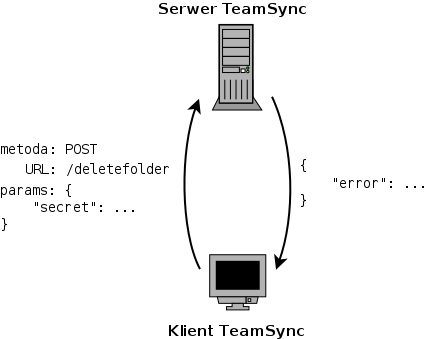
\includegraphics[width=240pt]{figures/metdeletefolder.png}
  \end{center}
  \caption{Komunikacja w systemie \emph{TeamSync} podczas wywoływania metody \texttt{addfolder} --- tworzenie folderu.}
  \label{picmetdeletefolder}
\end{figure}

Usuwanie katalogu odbywa się poprzez wysłanie do serwera żądania \texttt{HTTP} za pomocą metody \texttt{POST} na adres \texttt{http://<adres oraz port serwera TeamSync>\-/deletefolder}. Parametrem przesyłanym wewnątrz zapytania jest \emph{secret} folderu. Serwer nie robi nic poza przesłaniem \emph{secreta} za pomocą funkcji \texttt{remove\_folder} protokołu BitTorrent Sync API (dokładny opis funkcji \texttt{remove\_folder} w sekcji \ref{btsyncapiproto}) i  przekazuje odpowiedź --- o pomyślnym lub niepomyślnym usunięciu --- do klienta.

W przypadku niepowodzenia rola serwera kończy się na przekazaniu wyniku. Natomiast jeśli usunięcie folderu z listy synchronizowanych katalogów przebiegnie pomyślnie, serwer musi zmodyfikować plik konfiguracyjny \texttt{config.json} w celu usunięcia ze zmiennej \texttt{identities} tożsamości, której użytkownik już nie będzie potrzebował, ponieważ folder stanowiący jej środowisko przestał istnieć.

\subsection{Komentarze}

\label{comments}

Aplikacja TeamSync nie umożliwia usuwania komentarzy przez użytkowników nawet w przypadku gdy osobą, która chciałaby usunąć wypowiedź z systemu, jest jej autor. Usunięcie komentarza można zastąpić poprzez zmodyfikowanie lub całkowite usunięcie jego treści, natomiast obecność wypowiedzi w systemie będzie zawsze widoczna.

\subsubsection*{Czytanie komentarzy}

\begin{figure}[h!]
  \vspace{5pt}
  \begin{center}
    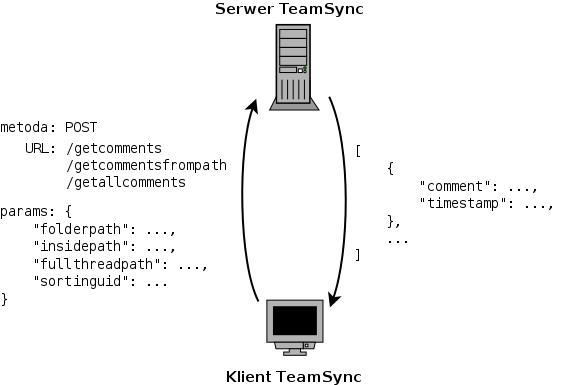
\includegraphics[width=320pt]{figures/metgetcomments.png}
  \end{center}
  \caption{Komunikacja w systemie \emph{TeamSync} podczas wywoływania metod \texttt{getcomments}, \texttt{getallcomments} oraz \texttt{getcommentsfrompath} --- czytanie komentarzy.}
  \label{picmetdeletefolder}
\end{figure}

Główną czynnością aplikacji TeamSync podczas wyświetlania komentarzy jest pobranie ich z serwera i przeniesienie odpowiedzi serwera do listy \texttt{comments}, która jest główną strukturą wyświetlaną w sekcji komentarzy. Zawiera ona komentarze w takiej strukturze, w jakiej są one przeczytane przez serwer z plików wewnątrz folderu z wątkiem.

Pobieranie listy komentarzy inicjowane jest z kodu \texttt{javascript} przeglądarki, a użyte do tego celu zapytania różnią się w zależności od widoku (aby zapoznać się dokładniej z widokami, należy przeczytać dodatek \ref{views}), w którym użytkownik aktualnie się znajduje:

\begin{description}[noitemsep]
  \item[W widoku nowego wątku] nie są pobierane żadne komentarze. W momencie wprowadzenia danych i zatwierdzenia nowego wątku system automatycznie przechodzi do widoku aktualnego wątku.
  
  \item[W widoku aktualnego wątku] odświeżanie listy komentarzy odbywa się za pomocą funkcji \texttt{re\-freshComments} wywoływanej np. podczas przechodzenia do nowego wątku albo wprowadzenia nowego komentarza. Jej zadaniem jest wysłanie na URL serwera \texttt{http://<adres oraz port serwera TeamSync>\-/getcomments} zapytania metodą \texttt{POST}, wewnątrz którego znajdują się następujące dane:
  \begin{itemize}[noitemsep]
    \item \emph{fullthreadpath} --- pełna ścieżka lokalizacji wątku, niezbędna do pobrania listy komentarzy,
    \item \emph{sortinguid} --- identyfikator użytkownika, według którego mają zostać posortowane komentarze. Jeśli wartość ta pozostanie pusta (domyślnie), serwer posortuje komentarze według ich znaczników czasowych pobranych w momencie umieszczenia ich w systemie TeamSync. W przeciwnym wypadku (\emph{sortinguid} wskazuje któregoś z użytkowników), wypowiedzi zostaną posortowane w takiej kolejności, w jakiej zostały odczytane przez wskazanego w argumencie \emph{sortinguid} użytkownika. Serwer wówczas --- zanim zwróci w odpowiedzi listę komentarzy --- posortuje dane według struktury \texttt{readby}, wewnątrz której umieszczone są znaczniki czasowe momentu odczytania wiadomości przez wskazanego użytkownika (sortowanie komentarzy według różnych spójności zostało szczegółowo opisane w sekcji \ref{consistencies}).
  \end{itemize}
  Jak zostało opisane na początku sekcji --- serwer odpowiada listą komentarzy odczytanych z plików i w zależności od zawartości argumentu \emph{sortinguid} sortuje wyjściowe dane przed ich wysłaniem do klienta.

  \item[W widoku bieżącej lokalizacji] do zmiennej \texttt{comments} zostaną przypisane komentarze z odpowiedzi serwera na zapytanie wysłane przez funkcję \texttt{getCommentsFromPath} uruchamianą w kodzie \texttt{javascript} przeglądarki klienta. Funkcja ta wysyła żądanie metodą \texttt{POST} na adres URL serwera \texttt{http://<adres oraz port serwera TeamSync>\-/getcommentsfrompath} z danymi w formacie JSON:
  \begin{itemize}[noitemsep]
    \item \emph{folderpath} --- bezwzględna ścieżka synchronizowanego folderu.
    \item \emph{insidepath} --- lokalizacja wewnątrz folderu, z której poziomu będą pobierane wszystkie komentarze. Nie będą brane pod uwagę komentarze w wątkach umieszczonych wewnątrz poziomów, wgłąb lokalizacji.
  \end{itemize}
  Konieczność wysłania dwóch ścieżek zamiast jednej podyktowana jest faktem, iż w przypadku pobierania komentarzy z jednego wątku zmienna \emph{fullthreadpath} zawarta jest --- obok innych informacji, np. nazwie, znaczniku czasowym powstania itd. --- w obiekcie wyświetlanym przez graficzny interfejs. Podczas pobierania komentarzy z jednego wątku wystarczy przekazać tą zmienną serwerowi. Natomiast w obecnym wypadku pobierania komentarzy z całej lokalizacji, nie ma jednego konkretnego wątku, z którego można by pozyskać tą informację, więc zostało przyjęte rozwiązanie, w którym klient wysyła dwie ścieżki, a serwer łączy je w całość (łącznie z katalogiem \texttt{.Comments} ścieżki łączone są na wzór \texttt{<folderpath>/.Comments/<insidepath>}) i dopiero z tak uzyskanej ścieżki pobierane są komentarze.
  
  \item[W widoku wszystkich komentarzy] w kodzie skryptu interfejsu uruchamiana jest nie przyjmująca żadnego argumentu funkcja \texttt{get\-All\-Comments}. Jej zadaniem jest wysłanie metodą \texttt{POST} na adres URL serwera \texttt{http://<adres oraz port serwera TeamSync>/getallcomments} bezwzględnej ścieżki synchronizowanego folderu. Serwer po jej odebraniu pobierze wszystkie komentarze napisane wewnątrz katalogu niezależnie od poziomu zagłębienia wewnątrz niego.
  
  \item[W widoku wszystkich komentarzy użytkownika] procedura uzyskiwania od serwera wyświetlanych postów wygląda identycznie jak w przypadku widoku wszystkich komentarzy. Jedyną różnicą w sposobie ich wyświetlania jest filtrowanie ich po stronie klienta według \emph{uid} autora wypowiedzi. Użytkownik wybierając autora, którego komentarze chciałby wyświetlić, w rzeczywistości pobiera wszystkie wypowiedzi z folderu i dopiero po ich uzyskaniu nakładany jest filtr. Dzięki takiemu podejściu możliwe jest szybsze oglądanie komentarzy różnych użytkowników, ponieważ pobierane one są raz. Zmieniając autora, zmieniane jest tylko filtrowanie wypowiedzi.
\end{description}

\subsubsection*{Pisanie komentarzy}

\begin{figure}[h!]
  \vspace{5pt}
  \begin{center}
    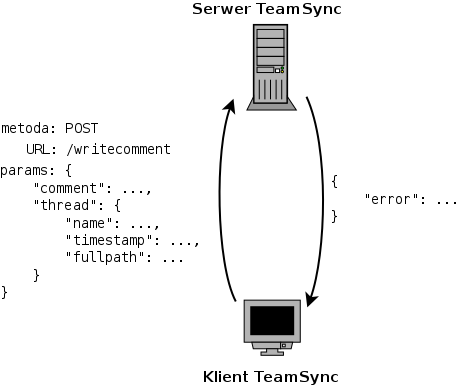
\includegraphics[width=250pt]{figures/metwritecomment.png}
  \end{center}
  \caption{Komunikacja w systemie \emph{TeamSync} podczas wywoływania metody \texttt{writecomment} --- pisanie komentarzy.}
  \label{picmetdeletefolder}
\end{figure}

Użytkownik przeglądając komentarze, może odpowiadać na nie tylko w przypadku, gdy przegląda je w widoku wątku (aby zapoznać się dokładniej z widokami, należy przeczytać dodatek \ref{views}). Nie ma możliwości odpisywania odpowiedzi na komentarz, nie znając kontekstu całego wątku, gdyż może to doprowadzić do nieporozumień między użytkownikami. Dlatego też możliwość komentowania we wszystkich widokach oprócz widoku wątku została zablokowana.

W widoku wątku --- na końcu konwersacji po obecnie ostatnim poście --- znajduje się pole tekstowe, gdzie użytkownik może wpisać treść swojej odpowiedzi, a następnie kliknąć przycisk, który metodą \texttt{POST} wysyła na adres \texttt{http://<adres oraz port serwera TeamSync>/\-writecomment} żądanie zawierające obiekt \texttt{JSON} z wartościami o następujących kluczach:

\begin{itemize}[noitemsep]
 \item \emph{comment} --- treść komentarza wpisana przez użytkownika,
 \item \emph{thread} --- obiekt JSON zawierający dane dotyczące aktywnego wątku (tego, w którym odpowiada użytkownik), które zawiera nastepujące informacje:
 \begin{itemize}[noitemsep]
  \item \emph{aaa} --- dsadsadasda
  \item \emph{dsadasdsa} --- dasczxczxcxz
 \end{itemize}
\end{itemize}

\begin{figure}[htb!]
\label{newcommentrequest}
  \begin{verbatim}
{
    "comment": "Treść nowego komentarza", 
    "thread": {
        "numberofcomments": 7, 
        "name": "Testowy tytul", 
        "timestamp": "1438513896000", 
        "lastcomment": "1439395572000", 
        "path": "/", 
        "fullpath": "/home/user/aaa/.Comments/1438513896000@#&$Testowy tytul", 
        "type": "thread", 
        "unreadcomment": false
    }
}
  \end{verbatim}
  \caption{Przykładowe żądanie wysyłane do serwera podczas odpowiedzi na wątek.}
\end{figure}

Po otrzymaniu od klienta żądania z tymi danymi serwer za pomocą ścieżki \texttt{fullpath} wewnątrz słownika \texttt{thread} pobierze z serwera NTP znacznik czasowy (aby uwiarygodnić przykład, założono, że pobrany znacznik czasowy to \texttt{1439396297000}) i umieści w podanej lokalizacji (\texttt{/home/\-user/\-aaa/\-.Comments/\-1438513896000\@\#\&\$Testowy tytul}) nowy plik z komentarzem o nazwie \texttt{1439396\-297000\@\#\&\$2HI7KRUNS\-SONIUJKM\-RWXGOTIZ\-SHBGFIH}:

\begin{figure}[htb]
\begin{verbatim}
           {
               "comment": "Treść nowego komentarza",
               "timestamp": "1439396297000",
               "history": [
                   {
                       "comment": "Treść nowego komentarza",
                       "timestamp": "1439396297000"
                   }
               ], 
               "uid": "2HI7KRUNSSONIUJKMRWXGOTIZSHBGFIH",
               "readby": {
                   "2HI7KRUNSSONIUJKMRWXGOTIZSHBGFIH": "1439395604000"
               }
           }
\end{verbatim}
  \caption{Plik komentarza zapisany w wyniku otrzymania przez serwer  wyżej zaprezentowanego żądania.}
\end{figure}

\subsubsection*{Edycja komentarzy}

\begin{figure}[h!]
  \vspace{5pt}
  \begin{center}
    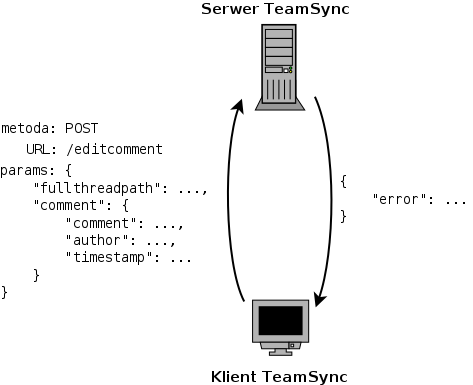
\includegraphics[width=260pt]{figures/meteditcomment.png}
  \end{center}
  \caption{Komunikacja w systemie \emph{TeamSync} podczas wywoływania metody \texttt{editcomment} --- edycja komentarzy.}
  \label{picmetdeletefolder}
\end{figure}

Modyfikacja komentarza może być dokonana tylko przez jego autora. Dzięki zastosowaniu takiego podejścia obniżone zostało ryzyko wystąpienia konfliktu podczas synchronizacji, ponieważ liczba osób mogących edytować plik komentarza została zredukowana do jednej.

Po zatwierdzeniu zmian do serwera wysyłane są dane niezbędne do odnalezienia komentarza w systemie plików i dopisania następnego wpisu do słownika \texttt{history} znajdującego się wewnątrz pliku z wypowiedzią wypowiedzi. Informacje wysyłane są za pomocą metody \texttt{POST} na adres \texttt{http://<adres oraz port\- serwera TeamSync>/\-editcomment}. Tymi danymi są:

\begin{itemize}[noitemsep]
  \item lokalizacja wątku --- pełna ścieżka folderu przechowującego pliki komentarzy oraz plik z metadanymi w dyskusji (plik \texttt{meta}),
  
  \item cały obiekt JSON zawierający dane komentarza w formie, w jakiej jest on odczytywany z pliku, z tą różnicą, że w zmiennej \texttt{comment} (zawierającej treść komentarza) znajduje się nowa, zmodyfikowana przez użytkownika wypowiedź.
\end{itemize}

Po otrzymaniu żądania zawierającego powyższe informacje serwer odtwarza tytuł pliku komentarza, posługując się zmiennymi \texttt{timestamp} oraz \texttt{uid}, otrzymując pełną ścieżkę komentarza. Wczytuje plik komentarza zapisany na dysku, modyfikuje zmienną \texttt{comment} treścią podaną przez użytkownika i dodaje do słownika \texttt{history} nowy element zawierający pobrany znacznik czasowy z serwera \emph{NTP} oraz nową treść wypowiedzi. Następnie zapisuje komentarz w tym samym pliku.

Aby zaoszczędzić czas, który tracony jest na odczytywanie pliku z systemu plików, serwer mógłby pominąć ten etap i --- po dodaniu wpisu do zmiennej \texttt{history} --- od razu komentarz zapisać. Jednak dane przesyłane z przeglądarki do serwera zawierają informacje nadmiarowe dotyczące interfejsu graficznego, które są zbędne dla serwera. Do poprawnego działania funkcji serwerowi wystarczyłyby dane:

\begin{itemize}[noitemsep]
  \item \emph{comment} --- nowa treść komentarza,
  
  \item \emph{timestamp} --- znacznik czasowy utworzenia komentarza (potrzebne do identyfikacji pliku w folderze wątku),
  
  \item \emph{uid} --- autor komentarza (potrzebne do identyfikacji pliku w folderze wątku),
  
  \item \emph{fullthreadpath} --- pełna ścieżka wątku, w którym komentarz jest fizycznie zapisany.
\end{itemize}

Jednakże zdecydowano się na przesłanie całej struktury komentarza ze względu na niewielką nadmiarowość danych oraz większe możliwości manipulacji zapisywaniem komentarza podczas ewentualnych ulepszeń aplikacji TeamSync w przyszłości.

\subsection{Wątki}

Użytkownicy mają możliwość tworzyć komentarze oraz je edytować, natomiast \emph{TeamSync} nie umożliwia usuwania ich ze względu na zachowanie spójności logicznej dyskusji. W przypadku wątków możliwości użytkowników zostały dodatkowo ograniczone --- edytowanie wątku zostało zminimalizowane wyłącznie do edycji treści pierwszego komentarza. Ze względu na fakt, iż była ona omówiona wcześniej (sekcja \ref{comments}), omówiona zostanie wyłącznie procedura dodawania do systemu nowej dyskusji.

\subsubsection*{Tworzenie nowego wątku}

\begin{figure}[h!]
  \vspace{5pt}
  \begin{center}
    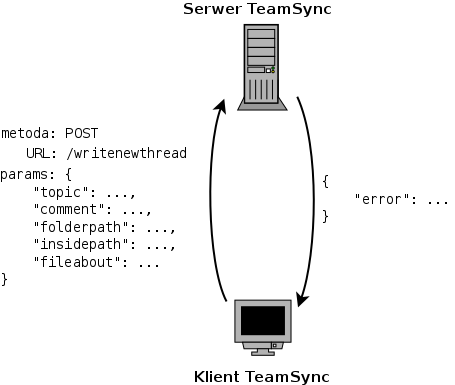
\includegraphics[width=250pt]{figures/metwritenewthread.png}
  \end{center}
  \caption{Komunikacja w systemie \emph{TeamSync} podczas wywoływania metody \texttt{writenewthread} --- tworzenie nowego watku.}
  \label{picmetdeletefolder}
\end{figure}

Użytkownik tworząc nowy wątek, wysyła --- poprzez aplikację kliencką w przeglądarce --- do serwera żądanie \texttt{HTTP} za pomocą metody \texttt{POST} na adres \texttt{http://<adres oraz port\- serwera TeamSync>/\-writenewthread}. W zapytaniu przesyłane sa następujące parametry:

\begin{itemize}[noitemsep]
  \item \emph{topic} --- tytuł wątku wprowadzony przez użytkownika,
  
  \item \emph{comment} --- treść pierwszego komentarza wprowadzona przez użytkownika,
  
  \item \emph{folderpath} --- bezwzględna ścieżka synchronizowanego folderu w lokalnym systemie operacyjnym użytkownika,
  
  \item \emph{insidepath} --- lokalizacja wątku wewnątrz folderu nie uwzględniając samego katalogu przechowującego wątek,
  
  \item \emph{fileabout} --- nazwa pliku wybranego przez użytkownika, którego dotyczyć będzie wątek.
\end{itemize}

Po otrzymaniu żądania serwer w pierwszej kolejności pobiera znacznik czasowy z serwera NTP, który jest potrzebny do wygenerowania nazwy folderu z nowym wątkiem łączącej ze sobą pobrany znacznik, identyfikator użytkownika oraz separator nazwy (dokładny opis separatora znajduje się w sekcji \ref{filenames}). Przyjmując jako separator użyty w implementacji ciąg znaków: \texttt{@\#\&\$}, nazwa katalogu wygląda następująco:

\begin{verbatim}
               < znacznik czasowy >@#&$< identyfikator użytkownika >
\end{verbatim}

Następnie serwer ustala pełną ścieżkę wątku z przekazanych w żądaniu parametrów \texttt{folderpath} oraz \texttt{insidepath}:

\begin{verbatim}
            folderpath/.Comments/insidepath/< nazwa katalogu z wątkiem >
\end{verbatim}

Po ustaleniu pełnej lokalizacji wątku serwer tworzy folder o podanej wyżej ścieżce i umieszcza w nim plik \texttt{meta} uzupełniając go wartościami podanymi przez użytkownika w żądaniu. Poniżej przedstawiono przykładowe parametry przesyłane w celu stworzenia nowego wątku w postaci obiektu \texttt{JSON}.

\begin{figure}[htb]
\begin{verbatim}
                {
                    "topic": "Testowy tytuł", 
                    "comment": "Przykładowa treść komentarza", 
                    "insidepath": "/abc", 
                    "fileabout": "aaa", 
                    "folderpath": "/home/user/testowy katalog"
                }
\end{verbatim}
  \caption{Parametry przesyłane w przykładowym zapytaniu tworzącym nowy wątek.}
\end{figure}

Według parametrów zawartych w przykładzie nowy wątek będzie miał tytuł \texttt{Testowy tytuł}, a treść pierwszego komentarza to \texttt{Przykładowa treść komentarza}. Lokalizacja uwspólnionego folderu, wewnątrz którego zamieszczany jest wątek, to \texttt{/home/user/\-testowy katalog}, natomiast wątek umieszczony jest jeden poziom głębiej, w katalogu \texttt{abc}. Dodatkowo utworzona dyskusja dotyczy pliku o pełnej ścieżce \texttt{/home/user/\-testowy katalog/\-abc/aaa}.

W wyniku otrzymania powyższego żądania --- zakładając, że pobrany znacznik czasowy to \texttt{1441566\-810000}, a identyfikator użytkownika zakładającego wątek to \texttt{FWZPQQKU\-E3JPQKWY5\-57FERJ4S\-D3BSFMM} --- serwer utworzy wątek w lokalizacji o pełnej ścieżce:

\begin{verbatim}
       /home/user/testowy katalog/.Comments/abc/
                         1441566810000@#&$FWZPQQKUE3JPQKWY557FERJ4SD3BSFMM
\end{verbatim}

Wewnątrz tego folderu zostanie umieszczony plik \texttt{meta} oraz plik pierwszego komentarza o podanych poniżej zawartościach.

\begin{figure}[htb]
\begin{verbatim}
                {
                    "topic": "Testowy tytuł", 
                    "timestamp": "1441566810000", 
                    "fileabout": "/abc/aaa", 
                    "uid": "FWZPQQKUE3JPQKWY557FERJ4SD3BSFMM"
                }
\end{verbatim}
  \caption{Zawartość pliku \texttt{meta} utworzonego w wyniku otrzymania przykładowego żądania.}
\end{figure}

\begin{figure}[htb]
\begin{verbatim}
           {
               "comment": "Przykładowa treść komentarza", 
               "timestamp": "1441566810000", 
               "history": [
                   {
                       "comment": "Przykładowa treść komentarza", 
                       "timestamp": "1441566810000"
                   }
               ], 
               "readby": {
                   "FWZPQQKUE3JPQKWY557FERJ4SD3BSFMM": "1441566810000"
               }, 
               "uid": "FWZPQQKUE3JPQKWY557FERJ4SD3BSFMM"
           }
\end{verbatim}
  \caption{Zawartość pliku z pierwszym komentarzem utworzonego w wyniku otrzymania przykładowego żądania.}
\end{figure}

W pliku \texttt{meta} zapisanym w folderze w wyniku otrzymania przez serwer przykładowego żądania umieszczony został tytuł \texttt{Testowy tytuł} wpisany przez użytkownika, znacznik czasowy zwrócony przez serwer NTP, identyfikator autora wątku oraz wewnętrzna ścieżka do pliku, na którego temat powstała dyskusja. Jeśli wątek nie dotyczyłby żadnego z plików, wartość \texttt{fileabout} byłaby równa \texttt{<brak>}.

Zapisywanie plików komentarzy zostało dokładniej opisane w sekcji \ref{comments}.

\section{Aplikacja przeglądarkowa}

Wśród podstawowych założeń implementacyjnych aplikacji \emph{TeamSync} --- poza założeniami wynikającymi z zastosowania systemu \emph{BitTorrent Sync} jako narzędzia odpowiedzialnego za wymianę danych --- znajdują się wymagania dotyczące interakcji człowieka z systemem. Podstawowymi założeniami --- oprócz prostoty interfejsu oraz łatwości jego obsługi --- w tym zakresie są: częstość odświeżania informacji oraz szybkość działania.

Aby sprostać powyższym wymaganiom i zachować interfejs w statycznym środowisku --- jakim jest serwer WWW --- zastosowano w pracy asynchroniczne zapytania (\emph{AJAX} \cite{ajax}) między częścią serwerową i kliencką. Podczas niemal każdej z czynności wykonywanych przez użytkownika w interfejsie odświeżana jest większa część danych pokazywanych użytkownikowi:

\begin{itemize}[noitemsep]
  \item komentarze,
  \item listy wątków,
  \item listy plików/katalogów przechowywanych w synchronizowanym folderze.
\end{itemize}

\subsubsection*{Two-way data binding}

Ważnym mechanizmem umożliwiającym dynamiczną zmianę treści strony unikając jej całkowitego przeładowania, jest tzw. ,,\emph{two-way data binding}'' zaimplementowany przez twórców narzędzia \emph{AngularJS}. Interfejs działający w tym systemie wyświetla elementy \emph{modelu}, które użytkownik zaimplementuje --- w przypadku aplikacji \emph{TeamSync} wewnątrz modelu znajdują się np. wszystkie listy przechowujące dane (listy plików, wątków, komentarzy, identyfikator użytkownika, itp.) albo ustawienia aplikacji.

Ogólna koncepcja metody ''\emph{two-way data binding}'' polega na zrealizowaniu jednocześnie dwóch następujących założeń dotyczących sposobu prezentacji w interfejsie danych pochodzących z modelu:

\begin{enumerate}[noitemsep]
  \item Jeśli dane zmienią się wewnątrz modelu, zmiana nastąpi również w interfejsie graficznym.
  
  \item Jeśli dane prezentowane w interfejsie graficznym zostaną zmienione, zmiana nastąpi również w \emph{modelu}.
\end{enumerate}

W ten sposób --- korzystając z pierwszego założenia --- jeśli wewnątrz kodu przeglądarki nastąpi odświeżenie dowolnej zmiennej (np. listy plików) poprzez zapytanie asynchroniczne, zostanie ona z natychmiastowym skutkiem zmieniona w interfejsie graficznym. Przykładem wykorzystania drugiego założenia może być sytuacja, w której użytkownik chce posortować wątki według żądanego kryterium. Wprowadzając odmienne kryterium niż obecne, wywołuje szereg operacji nie na zmiennych wyświetlanych w interfejsie, lecz na zmiennych wewnątrz modelu.

Dokładniejszy opis i przykłady obydwóch powyższych założeń zostaną przedstawione w następnych podrozdziałach.

\subsection{Wyświetlanie plików}

Podczas odświeżania listy plików, w kodzie \emph{javascript} interfejsu wysyłane jest asynchroniczne zapytanie metodą \texttt{POST}, a cała struktura, którą przeglądarka otrzyma w odpowiedzi od serwera, umieszczana jest wewnątrz zmiennej \texttt{files} reprezentującej listę plików. Aby przedstawić całą otrzymaną listę w interfejsie użytkownika, należy umieścić ją w strukturze, która umożliwi czytelne odwzorowanie listy. W tym celu posłużono się znacznikami \texttt{ul} oraz \texttt{li}, które są stworzone z myślą o prezentacji list (ul = unordered list). Przykładowe użycie znaczników \texttt{ul} oraz \texttt{li} wygląda następująco:

\begin{figure}[htb]
\begin{verbatim}
                            <ul>
                                <li>Element 1</li>
                                <li>Element 2</li>
                                <li>Element 3</li>
                            </ul>
\end{verbatim}
\end{figure}

\emph{AngularJS} umożliwia dynamiczną manipulację elementami listy poprzez dyrektywę \texttt{ng-repeat} dodawaną do tego znacznika, który ma zostać powtórzony. W przypadku powyższego przykładowego kodu dyrektywa \texttt{ng-repeat} zostanie dodana do pierwszego znacznika \texttt{li}. Jeśli w modelu istniałaby zmienna \texttt{list}, będąca tablicą zawierającą trzy elementy o typie znakowym: ,,\texttt{Element 1}'', ,,\texttt{Element 2}'' oraz ,,\texttt{Element 3}'', poniższy kod w pliku \emph{HTML} byłby jednakowy z wcześniejszym:

\begin{figure}[htb]
\begin{verbatim}
                 <ul>
                     <li ng-repeat="item in list">{{ item }}</li>
                 </ul>
\end{verbatim}
\end{figure}

Dyrektywa \texttt{ng-repeat} tworzy pętlę przechodzącą po wszystkich elementach listy, która wewnątrz każdego znacznika \texttt{li} umieszcza element, którego aktualnie dotyczy iteracja. Podwójny nawias ,,\{'' służy do umieszczania zawartości przechowywanych wewnątrz zmiennych, które służą jako iterator (w powyższym przypadku iteratorem jest zmienna \texttt{item}).Jeśli modyfikacji (na przykład podczas asynchronicznego zapytania do serwera i zaktualizowania listy) ulegnie lista \texttt{list}, wewnątrz której odbywa się iteracja w dyrektywie \texttt{ng-repeat}, zmiana zostanie przeniesiona na interfejs. Spełnione zostanie pierwsze założenie metody \emph{two-way data binding} --- zmiana modelu wpłynie na interfejs graficzny.

Dyrektywa \texttt{ng-repeat} została wykorzystana w aplikacji \emph{TeamSync} np. do prezentowania listy plików. Zmienna \texttt{files}, w której umieszczane są elementy pochodzące z odpowiedzi serwera, stanowi listę, wewnątrz której dyrektywa \texttt{ng-repeat} iteruje, wyświetlając odpowiednie informacje użytkownikowi.

\begin{figure}[htb]
\begin{verbatim}
           <ul>
               <li ng-repeat="file in files">{{ file.name }}</li>
           </ul>
\end{verbatim}
\end{figure}

Ze względu na założenia metody \emph{two-way data binding}, w momencie odebrania odpowiedzi od serwera, przeglądarka natychmiast wyświetli aktualną listę plików, czego efektem jest niezbędna dynamika aplikacji. Ponieważ zawarte wewnątrz listy \texttt{files} elementy są obiektami \texttt{JSON}, wewnątrz podwójnych nawiasów klamrowych musiała zostać umieszczona któraś z wartości obiektu, a nie cały obiekt. Skoro użytkownik musi widzieć nazwę pliku, aby móc nawigować po synchronizowanym folderze, została użyta wartość obiektu \texttt{file}, której kluczem jest \texttt{name} (nazwa).

W podobny sposób działają wszystkie dynamiczne elementy strony interfejsu graficznego, które są modyfikowane zarówno przez serwer, jak i użytkownika. Przykładem zmiennych, które prezentowane sa w podobny sposób do plików, są:

\begin{itemize}[noitemsep]
  \item lista folderów,
  \item lista wszystkich użytkowników w folderze,
  \item lista komentarzy,
  \item lista wątków.
\end{itemize}


\subsection{Filtrowanie komentarzy}

Wyszukiwanie wewnątrz komentarzy wpisywanych przez użytkownika fraz w aplikacji \emph{TeamSync} odbywa się w całości po stronie klienta, dzięki czemu jest bardzo szybkie i dynamiczne. Filtr jest uaktualniany i zaczyna działać podczas wprowadzenia każdego znaku. Odbywa się to dzięki użyciu słowa kluczowego \texttt{filter} dostępnego w systemie \emph{AngularJS}, którego umieszczenie w odpowiedni sposób wewnątrz kodu HTML aplikacji spowoduje wykluczenie ze zbioru danych elementów niepasujących do wzorca.

Użycie funkcji \texttt{filter} zostanie opisane na kodzie HTML z wcześniejszego przykładu, do którego dodano funkcjonalność filtrowania:

\begin{figure}[htb]
\begin{verbatim}
      <ul>
          <li ng-repeat="item in list | filter:testFilter">{{ item }}</li>
      </ul>
\end{verbatim}
\end{figure}

Znak ,,\texttt{|}'' jest znakiem, który powoduje poddanie zbioru danych sprzed tego znaku (w tym przykładzie jest to lista \texttt{list}) działaniu operacji po tym znaku --- filtrowaniu, lub sortowaniu (w tym przykładzie jest to filtrowanie). Słowo \texttt{filter} jest słowem kluczowym oznaczającym wykonywanie filtrowania na zbiorze danych \texttt{list}. \texttt{testFilter} jest zmienną pochodzącą z modelu, wewnątrz której przechowywana jest wartość filtru. Jeśli byłby spełnione poniższe warunki:

\begin{figure}[htb]
\begin{verbatim}
               testFilter = "1"
               list = ["Element 1", "Element 2", "Element 3"]
\end{verbatim}
\end{figure}

Wewnątrz znacznika \texttt{ul} zostałyby wyświetlone wyłącznie te elementy \texttt{li}, których zawartość zawierałaby znak ,,$1$''. Posługując się obecnym przykładem, użytkownik wyświetlając powyższy kod z powyższymi danymi wewnątrz modelu zobaczyłby w swojej przeglądarce wyłącznie pierwszy element o treści \texttt{Element 1}.

Wewnątrz aplikacji \emph{TeamSync} funkcjonalność słowa kluczowego \texttt{filter} została wykorzystana do filtrowania tresci komentarzy w poszukiwaniu żądanego przez użytkownika słowa. Wszystkie komentarze aktualnie wyświetlane na ekranie zostają poddawane filtracji w poszukiwaniu wprowadzonej frazy. W uproszczonej wersji kod HTML tej funkcjonalności w aplikacji \emph{TeamSync} wygląda w następujący sposób:

\begin{figure}[htb]
\begin{verbatim}
         <ul>
             <li ng-repeat="comment in comments | filter: searchphrase">
         </ul>
\end{verbatim}
\end{figure}

Zmienna \texttt{comments} jest listą, do której asynchronicznie pobierane są z serwera komentarze w formie obiektów \texttt{JSON}. Podobnie jak w wyświetlaniu plików, również tutaj podczas aktualizacji tej zmiennej w modelu (dzięki technice \emph{two-way data binding}) natychmiast aktualizowane są elementy w interfejsie graficznym. Po słowie kluczowym \texttt{filter} --- sygnalizującym działanie filtra zbioru danych \texttt{comments} --- znajduje się zmienna \texttt{searchphrase}, której wartość jest ciągiem znaków wyszukiwanym wśród komentarzy. Wyświetlany zbiór wypowiedzi (spośród listy \texttt{comments}) zostanie ograniczony tylko do tych, które zawierają frazę wpisaną do zmiennej \texttt{searchphrase}.

Podczas tej operacji system \emph{AngularJS} skorzysta z drugiego założenia metody \emph{two-way data binding} --- użytkownik wprowadzając w interfejsie graficznym szukaną frazę, automatycznie uaktualni zmienną \texttt{searchphrase} w modelu. Z kolei zmienna \texttt{searchphrase} pobrana z modelu zostanie użyta do wyświetlenia zubożonego zbioru komentarzy o te, które nie pasują do wpisanego wzorca.

W systemie \emph{AngularJS} możliwe jest stosowanie wielu filtrów na tym samym zbiorze danych. W aplikacji \emph{TeamSync} zostało to wykorzystane, aby dodatkowo móc wyfiltrować te wiadomości, które zostały umieszczone przez konkretnych użytkowników.